\section{Specyfikacja przypadków użycia - poziom rozszerzony}
\newcommand{\myparagraph}[1]{\paragraph{#1}\mbox{}\\}

\subsection{Aktorzy}
\begin{itemize}
\item Użytkownik zasobów - osoba uprawniona jedynie do przeglądania zasobów zarejestrowanych w systemie
\item Administrator zasobów - osoba zarządzająca wprowadzonymi zasobami - dodaje, edytuje i usuwa zasoby, wprowadza także informacje nt. osób odpowiedzialnych za zasoby oraz rejestrujący użytkowników zasobu.
\item Serwisant - osoba odpowiedzialna za wprowadzanie informacji dotyczących napraw sprzętu, aktualizacji oprogramowania oraz operacji serwisowych.
\item Menadżer - osoba mająca możliwość generowania raportów przedstawiających statystyki nt. zasobów zarejestrowanych w systemie.
\end{itemize}


\subsection{PU1 Wyszukiwanie zasobów} \label{pu1}

\begin{figure}[h!]
	\centering
	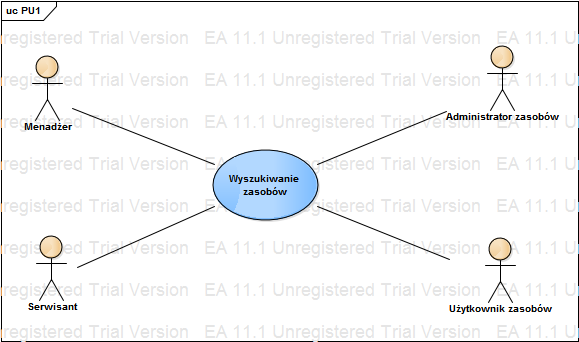
\includegraphics[scale=0.6]{img/diagrams/useCaseDiagrams/PU1.png}
	\caption{Diagram przypadku użycia PU1 \label{fig:labelUCPU1}}
\end{figure}

\myparagraph{Opis}
Przypadek wyszukiwania zasobów za pomocą zadanych kryteriów przez użytkownika.

\myparagraph{Aktorzy}
Jeden z następujących:
\begin{itemize}
\item użytkownik zasobów,
\item administrator zasobów,
\item menadżer,
\item serwisant.
\end{itemize}

\myparagraph{Warunki wstępne}
\begin{itemize}
\item Użytkownik jest zalogowany w systemie.
\end{itemize}

\myparagraph{Warunki końcowe}
Przypadek użycia nie wpływa na stan systemu.

\myparagraph{Przebieg podstawowy}
\begin{enumerate}
\item \label{pu1:f} Aktor wybiera ikonę wyszukiwania zasobów.
\item \label{pu1:s}System prezentuje okno wyszukiwania zasobów zawierające sekcję podawania kryteriów.
\item Aktor wprowadza kryteria wyszukiwania.
\item Aktor wciska przycisk ,,Wyszukaj''.
\item System prezentuje wyniki wyszukiwania.
\end{enumerate}

\myparagraph{Alternatywne przebiegi zdarzeń}
\begin{enumerate}
\item Aktor nie podał kryteriów wyszukiwania
	\begin{enumerate}[label*=\arabic*.]
	\item Kroki \ref{pu1:f} - \ref{pu1:s} jak w przebiegu podstawowym.
	\item Aktor wciska przycisk ,,Wyszukaj''.
	\item System wyświetla informację o konieczności podania kryteriów wyszukiwania.
	\end{enumerate}
\end{enumerate}

\myparagraph{Sytuacje wyjątkowe}
Brak połączenia z siecią.



\subsection{PU2 Obsługa sprzetu kopmuterowego} \label{pu2}

\begin{figure}[h!]
	\centering
	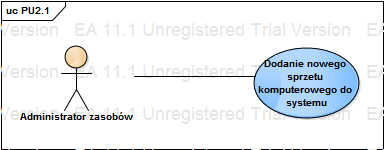
\includegraphics[scale=0.6]{img/diagrams/useCaseDiagrams/PU2_1.png}
	\caption{Diagram przypadku użycia PU2.1 \label{fig:labelUCPU2.1}}
\end{figure}

\begin{figure}[h!]
	\centering
	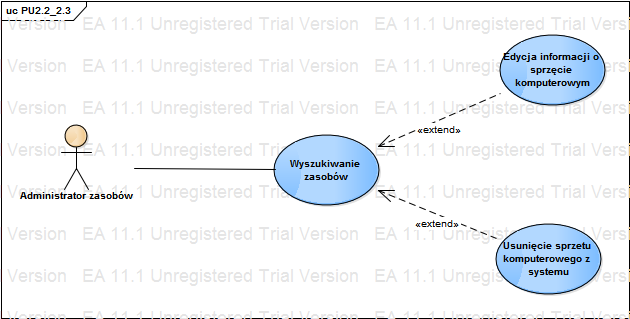
\includegraphics[scale=0.6]{img/diagrams/useCaseDiagrams/PU2_2_2_3.png}
	\caption{Diagram przypadków użycia PU2.2 i PU2.3 \label{fig:labelUCPU2.2_2.3}}
\end{figure}

\subsubsection{PU2.1 Dodanie nowego sprzętu komputerowego do systemu}

\myparagraph{Opis}
Przypadek dodawania nowego sprzętu komputerowego do systemu katalogowego.

\myparagraph{Aktorzy}
Administrator zasobów.

\myparagraph{Warunki wstępne}
\begin{itemize}
\item Użytkownik jest zalogowany w systemie.
\end{itemize}

\myparagraph{Warunki końcowe}
\begin{itemize}
\item Do systemu katalogowego został dodany nowy sprzęt komputerowy.
\end{itemize}

\myparagraph{Przebieg podstawowy}
\begin{enumerate}
\item \label{pu2.1:1} Aktor wybiera ikonę dodawania sprzętu komputerowego.
\item System prezentuje okno dodawania sprzętu komputerowego.
\item Aktor podaje dane dodawanego zasobu.
\item \label{pu2.1:4} Aktor wciska przycisk ,,Dodaj''.
\item System wyświetla potwierdzenie dodania sprzętu komputerowego do systemu.
\end{enumerate}

\myparagraph{Alternatywne przebiegi zdarzeń}
\begin{enumerate}
\item Aktor nie posiada wystarczających uprawnień do dodania sprzętu komputerowego.
	\begin{enumerate}[label*=\arabic*.]
		\item Krok \ref{pu2.1:1} jak w przebiegu podstawowym.
		\item System wyświetla informację o brak wymaganych uprawnień.
	\end{enumerate}
\item Aktor podał niepoprawne lub niepełne dane sprzętu komputerowego.
	\begin{enumerate}[label*=\arabic*.]
		\item Kroki \ref{pu2.1:1} - \ref{pu2.1:4} jak w przebiegu podstawowym.
		\item System wyświetla informację o konieczności poprawienia danych.
	\end{enumerate}
\end{enumerate}

\myparagraph{Sytuacje wyjątkowe}
Brak połączenia z siecią.



\subsubsection{PU2.2 Edycja informacji o sprzęcie komputerowym}

\myparagraph{Opis}
Przypadek edycji danych sprzętu komputerowego znajdującego się w systemie katalogowym.

\myparagraph{Aktorzy}
Administrator zasobów.

\myparagraph{Warunki wstępne}
\begin{itemize}
\item Użytkownik jest zalogowany w systemie.
\item Sprzęt komputerowy istnieje w systemie katalogowym.
\end{itemize}

\myparagraph{Warunki końcowe}
\begin{itemize}
\item Dane sprzętu komputerowego zostały zmienione.
\end{itemize}

\myparagraph{Przebieg podstawowy}
\begin{enumerate}
\item \label{pu2.2:1} Aktor wyszukuje sprzęt zgodnie z \ref{pu1}
\item \label{pu2.2:2} Aktor wybiera sprzęt do edycji oraz wciska przycisk ,,Edytuj''.
\item System prezentuje okno edycji danych sprzętu komputerowego.
\item Aktor wprowadza nowe dane.
\item \label{pu2.2:5} Aktor wciska przycisk ,,Zapisz''.
\item System wyświetla potwierdzenie zmiany danych sprzętu komputerowego.
\end{enumerate}

\myparagraph{Alternatywne przebiegi zdarzeń}
\begin{enumerate}
\item Aktor nie posiada uprawnień do edycji danych sprzętu komputerowego.
	\begin{enumerate}[label*=\arabic*.]
		\item Kroki \ref{pu2.2:1} - \ref{pu2.2:2} jak w przebiegu podstawowym.
		\item System wyświetla informację o braku uprawnień do edycji.
	\end{enumerate}
\item Aktor podał niepoprawne lub niepełne dane sprzętu komputerowego.
	\begin{enumerate}[label*=\arabic*.]
		\item Kroki \ref{pu2.2:1} - \ref{pu2.2:5} jak w przebiegu podstawowym.
		\item System wyświetla informację o konieczności poprawienia danych.
	\end{enumerate}
\end{enumerate}

\myparagraph{Sytuacje wyjątkowe}\
Brak połączenia z siecią.

\subsubsection{PU2.3 Usunięcie sprzętu komputerowego z systemu}

\myparagraph{Opis}
Przypadek użycia opisuje procedurę usunięcia sprzętu komputerowego z systemu katalogowego.

\myparagraph{Aktorzy}
Administrator zasobów.

\myparagraph{Warunki wstępne}
\begin{itemize}
\item Użytkownik jest zalogowany w systemie.
\item Sprzęt komputerowy istnieje w systemie katalogowym.
\end{itemize}

\myparagraph{Warunki końcowe}
\begin{itemize}
\item Sprzęt komputerowy został usunięty z systemu katalogowego.
\end{itemize}

\myparagraph{Przebieg podstawowy}
\begin{enumerate}
\item \label{pu2.3:1} Aktor wyszukuje sprzęt zgodnie z \ref{pu1}
\item \label{pu2.3:2} Aktor wybiera sprzęt do usunięcia oraz wciska przycisk ,,Usuń''.
\item System wyświetla okno z prośbą o potwierdzenie wykonania operacji.
\item Aktor potwierdza wykonanie operacji.
\item System wyświetla potwierdzenie usunięcia sprzętu komputerowego z systemu.
\end{enumerate}

\myparagraph{Alternatywne przebiegi zdarzeń}
\begin{enumerate}
\item Aktor nie posiada uprawnień do usunięcia sprzętu komputerowego z systemu.
	\begin{enumerate}[label*=\arabic*.]
		\item Kroki \ref{pu2.3:1} - \ref{pu2.3:2} jak w przebiegu podstawowym.
		\item System wyświetla informację o braku uprawnień do usunięcia sprzętu komputerowego.
	\end{enumerate}
\end{enumerate}

\myparagraph{Sytuacje wyjątkowe}\
Brak połączenia z siecią.

\subsection{PU3 Obsługa oprogramowania} \label{pu3}

\begin{figure}[h!]
	\centering
	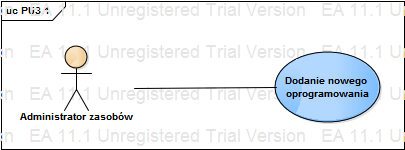
\includegraphics[scale=0.6]{img/diagrams/useCaseDiagrams/PU3_1.png}
	\caption{Diagram przypadku użycia PU3.1 \label{fig:labelUCPU3.1}}
\end{figure}

\begin{figure}[h!]
	\centering
	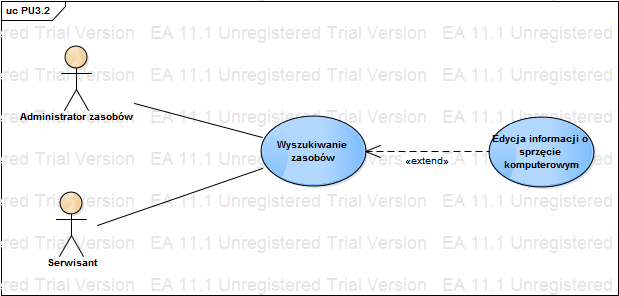
\includegraphics[scale=0.6]{img/diagrams/useCaseDiagrams/PU3_2.png}
	\caption{Diagram przypadku użycia PU3.2 \label{fig:labelUCPU3.2}}
\end{figure}

\begin{figure}[h!]
	\centering
	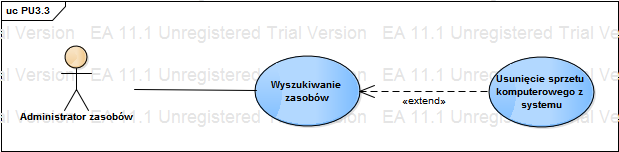
\includegraphics[scale=0.6]{img/diagrams/useCaseDiagrams/PU3_3.png}
	\caption{Diagram przypadku użycia PU3.3 \label{fig:labelUCPU3.3}}
\end{figure}

\subsubsection{PU3.1 Dodanie nowego oprogramowania}

\myparagraph{Opis}
Przypadek użycia opisuje procedurę dodania nowego oprogramowania do systemu katalogowego.

\myparagraph{Aktorzy}
Administrator zasobów.

\myparagraph{Warunki wstępne}
\begin{itemize}
\item Użytkownik jest zalogowany w systemie.
\end{itemize}

\myparagraph{Warunki końcowe}
\begin{itemize}
\item Oprogramowanie (wraz z danymi instalacji) zostało zapisane w systemie katalogowym.
\end{itemize}

\myparagraph{Przebieg podstawowy}
\begin{enumerate}
\item \label{pu3.1:1} Aktor wybiera ikonę dodawania oprogramowania.
\item System prezentuje okno dodawania oprogramowania.
\item Aktor podaje dane dodawanego zasobu wraz z informacjami na temat przeprowadzonych instalacji.
\item \label{pu3.1:4} Aktor wciska przycisk ,,Dodaj''.
\item System wyświetla potwierdzenie dodania oprogramowania do systemu katalogowego.
\end{enumerate}

\myparagraph{Alternatywne przebiegi zdarzeń}
\begin{enumerate}
\item Aktor nie posiada uprawnień do dodania oprogramowania.
	\begin{enumerate}[label*=\arabic*.]
		\item Krok \ref{pu3.1:1} jak w przebiegu podstawowym.
		\item System wyświetla informację o braku uprawnień do wykonania operacji dodania oprogramowania.
	\end{enumerate}
\item Aktor podał niepoprawne lub niepełne dane.
	\begin{enumerate}[label*=\arabic*.]
		\item Kroki \ref{pu3.1:1} - \ref{pu3.1:4} jak w przebiegu podstawowym.
		\item System wyświetla informację o konieczności poprawienia danych.
	\end{enumerate}
\end{enumerate}

\myparagraph{Sytuacje wyjątkowe}
Brak połączenia z siecią.

\subsubsection{PU3.2 Edycja informacji oprogramowaniu}

\myparagraph{Opis}
Przypadek użycia opisuje procedurę edycji informacji dotyczących oprogramowania znajdującego się w systemie - możliwa jest zmiana podstawowych danych oraz edycja przeprowadzonych instalacji.

\myparagraph{Aktorzy}
Administrator zasobów lub Serwisant.

\myparagraph{Warunki wstępne}
\begin{itemize}
\item Użytkownik jest zalogowany w systemie.
\item Oprogramowanie istnieje w systemie katalogowym.
\end{itemize}

\myparagraph{Warunki końcowe}
\begin{itemize}
\item Dane oprogramowania zostały zmienione.
\end{itemize}

\myparagraph{Przebieg podstawowy}
\begin{enumerate}
\item \label{pu3.2:1} Aktor wyszukuje oprogramowanie zgodnie z \ref{pu1}
\item \label{pu3.2:2} Aktor wybiera oprogramowanie do edycji oraz wciska przycisk ,,Edytuj''.
\item System prezentuje okno edycji danych oprogramowania.
\item Aktor wprowadza nowe dane.
\item \label{pu3.2:5} Aktor wciska przycisk ,,Zapisz''.
\item System wyświetla potwierdzenie zmiany danych oprogramowania.
\end{enumerate}

\myparagraph{Alternatywne przebiegi zdarzeń}
\begin{enumerate}
\item Aktor nie posiada uprawnień do edycji danych oprogramowania.
	\begin{enumerate}[label*=\arabic*.]
		\item Kroki \ref{pu3.2:1} - \ref{pu3.2:2} jak w przebiegu podstawowym.
		\item System wyświetla informację o braku uprawnień do edycji.
	\end{enumerate}
\item Aktor podał niepoprawne lub niepełne dane oprogramowania.
	\begin{enumerate}[label*=\arabic*.]
		\item Kroki \ref{pu3.2:1} - \ref{pu3.2:5} jak w przebiegu podstawowym.
		\item System wyświetla informację o konieczności poprawienia danych.
	\end{enumerate}
\end{enumerate}

\myparagraph{Sytuacje wyjątkowe}\
Brak połączenia z siecią.

\subsubsection{PU3.3 Usunięcie oprogramowania z systemu}

\myparagraph{Opis}
Przypadek użycia opisuje procedurę usunięcia oprogramowania (wraz z danymi na temat przeprowadzonych instalacji) z systemu katalogowego.

\myparagraph{Aktorzy}
Administrator zasobów.

\myparagraph{Warunki wstępne}
\begin{itemize}
\item Użytkownik jest zalogowany w systemie.
\item Oprogramowanie istnieje w systemie katalogowym.
\end{itemize}

\myparagraph{Warunki końcowe}
\begin{itemize}
\item Oprogramowanie zostało usunięte z systemu katalogowego.
\end{itemize}

\myparagraph{Przebieg podstawowy}
\begin{enumerate}
\item \label{pu3.3:1} Aktor wyszukuje sprzęt zgodnie z \ref{pu1}
\item \label{pu3.3:2} Aktor wybiera oprogramowanie oraz wciska przycisk ,,Usuń''.
\item System wyświetla okno z prośbą o potwierdzenie wykonania operacji.
\item Aktor potwierdza wykonanie operacji.
\item System wyświetla potwierdzenie usunięcia oprogramowania z systemu.
\end{enumerate}

\myparagraph{Alternatywne przebiegi zdarzeń}
\begin{enumerate}
\item Aktor nie posiada uprawnień do usunięcia oprogramowania z systemu.
	\begin{enumerate}[label*=\arabic*.]
		\item Kroki \ref{pu3.3:1} - \ref{pu3.3:2} jak w przebiegu podstawowym.
		\item System wyświetla informację o braku uprawnień do usunięcia oprogramowania.
	\end{enumerate}
\end{enumerate}

\myparagraph{Sytuacje wyjątkowe}\
Brak połączenia z siecią.

\subsection{PU4 Obsługa innego sprzętu, urządzeń lub wyposażenia} \label{pu4}

\begin{figure}[h!]
	\centering
	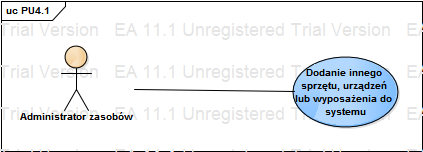
\includegraphics[scale=0.6]{img/diagrams/useCaseDiagrams/PU4_1.png}
	\caption{Diagram przypadku użycia PU4.1 \label{fig:labelUCPU2.1}}
\end{figure}

\begin{figure}[h!]
	\centering
	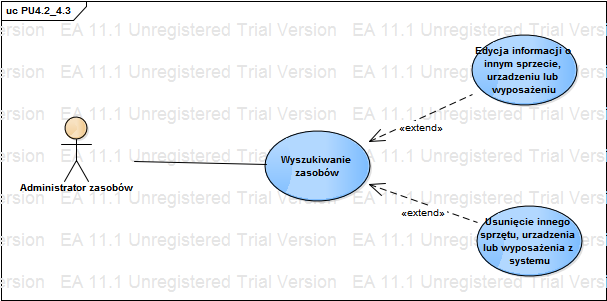
\includegraphics[scale=0.6]{img/diagrams/useCaseDiagrams/PU4_2_4_3.png}
	\caption{Diagram przypadków użycia PU4.2 i PU4.3 \label{fig:labelUCPU4.2_4.3}}
\end{figure}

\subsubsection{PU4.1 Dodanie innego sprzętu, urządzeń lub wyposażenia do systemu}

\myparagraph{Opis}
Przypadek użycia opisuje procedurę dodania sprzętu, urządzeń lub wyposażenia do systemu.

\myparagraph{Aktorzy}
Administrator zasobów.

\myparagraph{Warunki wstępne}
\begin{itemize}
\item Użytkownik jest zalogowany w systemie.
\end{itemize}

\myparagraph{Warunki końcowe}
\begin{itemize}
\item Zasób (wraz z danymi instalacji) został zapisany w systemie katalogowym.
\end{itemize}

\myparagraph{Przebieg podstawowy}
\begin{enumerate}
\item \label{pu4.1:1} Aktor wybiera ikonę dodawania zasobu.
\item System prezentuje okno dodawania zasobu.
\item Aktor podaje dane dodawanego zasobu.
\item \label{pu4.1:4} Aktor wciska przycisk ,,Dodaj''.
\item System wyświetla potwierdzenie dodania zasobu do systemu katalogowego.
\end{enumerate}

\myparagraph{Alternatywne przebiegi zdarzeń}
\begin{enumerate}
\item Aktor nie posiada uprawnień do dodania zasobu.
	\begin{enumerate}[label*=\arabic*.]
		\item Krok \ref{pu4.1:1} jak w przebiegu podstawowym.
		\item System wyświetla informację o braku uprawnień do wykonania operacji dodania zasobu.
	\end{enumerate}
\item Aktor podał niepoprawne lub niepełne dane.
	\begin{enumerate}[label*=\arabic*.]
		\item Kroki \ref{pu4.1:1} - \ref{pu4.1:4} jak w przebiegu podstawowym.
		\item System wyświetla informację o konieczności poprawienia danych.
	\end{enumerate}
\end{enumerate}

\myparagraph{Sytuacje wyjątkowe}
Brak połączenia z siecią.

\subsubsection{PU4.2 Edycja informacji o innym sprzęcie, urządzeniu lub wyposażeniu}

\myparagraph{Opis}
Przypadek użycia opisuje procedurę edycji informacji dotyczących ogólnych zasobów.

\myparagraph{Aktorzy}
Administrator zasobów.

\myparagraph{Warunki wstępne}
\begin{itemize}
\item Użytkownik jest zalogowany w systemie.
\item Zasób istnieje w systemie katalogowym.
\end{itemize}

\myparagraph{Warunki końcowe}
\begin{itemize}
\item Dane zasobu zostały zmienione.
\end{itemize}

\myparagraph{Przebieg podstawowy}
\begin{enumerate}
\item \label{pu4.2:1} Aktor wyszukuje zasób zgodnie z \ref{pu1}
\item \label{pu4.2:2} Aktor wybiera zasób do edycji oraz wciska przycisk ,,Edytuj''.
\item System prezentuje okno edycji danych zasobu.
\item Aktor wprowadza nowe dane.
\item \label{pu4.2:5} Aktor wciska przycisk ,,Zapisz''.
\item System wyświetla potwierdzenie zmiany danych zasobu.
\end{enumerate}

\myparagraph{Alternatywne przebiegi zdarzeń}
\begin{enumerate}
\item Aktor nie posiada uprawnień do edycji danych zasobu.
	\begin{enumerate}[label*=\arabic*.]
		\item Kroki \ref{pu4.2:1} - \ref{pu4.2:2} jak w przebiegu podstawowym.
		\item System wyświetla informację o braku uprawnień do edycji.
	\end{enumerate}
\item Aktor podał niepoprawne lub niepełne dane oprogramowania.
	\begin{enumerate}[label*=\arabic*.]
		\item Kroki \ref{pu4.2:1} - \ref{pu4.2:5} jak w przebiegu podstawowym.
		\item System wyświetla informację o konieczności poprawienia danych.
	\end{enumerate}
\end{enumerate}

\myparagraph{Sytuacje wyjątkowe}\
Brak połączenia z siecią.

\subsubsection{PU4.3 Usunięcie innego sprzętu, urządzenia lub wyposażenia z systemu}

\myparagraph{Opis}
Przypadek użycia opisuje procedurę usunięcia zasobu (ogólnego typu) z systemu katalogowego.

\myparagraph{Aktorzy}
Administrator zasobów.

\myparagraph{Warunki wstępne}
\begin{itemize}
\item Użytkownik jest zalogowany w systemie.
\item Zasób istnieje w systemie katalogowym.
\end{itemize}

\myparagraph{Warunki końcowe}
\begin{itemize}
\item Zasób został usunięty z systemu katalogowego.
\end{itemize}

\myparagraph{Przebieg podstawowy}
\begin{enumerate}
\item \label{pu4.3:1} Aktor wyszukuje zasób zgodnie z \ref{pu1}
\item \label{pu4.3:2} Aktor wybiera zasób oraz wciska przycisk ,,Usuń''.
\item System wyświetla okno z prośbą o potwierdzenie wykonania operacji.
\item Aktor potwierdza wykonanie operacji.
\item System wyświetla potwierdzenie usunięcia zasobu z systemu.
\end{enumerate}

\myparagraph{Alternatywne przebiegi zdarzeń}
\begin{enumerate}
\item Aktor nie posiada uprawnień do usunięcia zasobu z systemu.
	\begin{enumerate}[label*=\arabic*.]
		\item Kroki \ref{pu4.3:1} - \ref{pu4.3:2} jak w przebiegu podstawowym.
		\item System wyświetla informację o braku uprawnień do usunięcia zasobu.
	\end{enumerate}
\end{enumerate}

\myparagraph{Sytuacje wyjątkowe}\
Brak połączenia z siecią.

\subsection{PU5 Obsługa czasopisma lub zasobu literaturowego} \label{pu5}

\begin{figure}[h!]
	\centering
	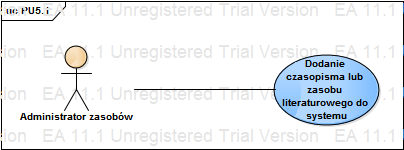
\includegraphics[scale=0.6]{img/diagrams/useCaseDiagrams/PU5_1.png}
	\caption{Diagram przypadku użycia PU5.1 \label{fig:labelUCPU5.1}}
\end{figure}

\begin{figure}[h!]
	\centering
	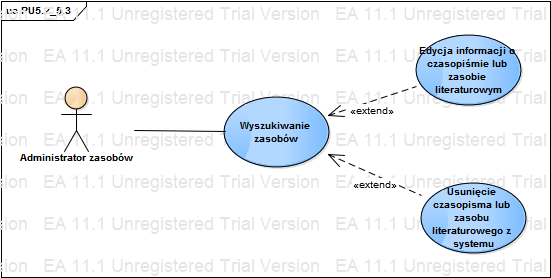
\includegraphics[scale=0.6]{img/diagrams/useCaseDiagrams/PU5_2_5_3.png}
	\caption{Diagram przypadków użycia PU5.2 i PU5.3 \label{fig:labelUCPU5.2_5.3}}
\end{figure}

\subsubsection{PU5.1 Dodanie nowego czasopisma lub zasobu literaturowego do systemu}

\myparagraph{Opis}
Przypadek użycia opisuje procedurę dodania czasopisma bądź zasobu literaturowego do systemu.

\myparagraph{Aktorzy}
Administrator zasobów.

\myparagraph{Warunki wstępne}
\begin{itemize}
\item Użytkownik jest zalogowany w systemie.
\end{itemize}

\myparagraph{Warunki końcowe}
\begin{itemize}
\item Dane czasopisma lub zasobu literackiego zostały zapisane w systemie katalogowym.
\end{itemize}

\myparagraph{Przebieg podstawowy}
\begin{enumerate}
\item \label{pu5.1:1} Aktor wybiera ikonę dodawania czasopisma/zasobu literaturowego.
\item System prezentuje okno dodawania zasobu.
\item Aktor podaje dane dodawanego zasobu.
\item \label{pu5.1:4} Aktor wciska przycisk ,,Dodaj''.
\item System wyświetla potwierdzenie dodania zasobu do systemu katalogowego.
\end{enumerate}

\myparagraph{Alternatywne przebiegi zdarzeń}
\begin{enumerate}
\item Aktor nie posiada uprawnień do dodania zasobu.
	\begin{enumerate}[label*=\arabic*.]
		\item Krok \ref{pu5.1:1} jak w przebiegu podstawowym.
		\item System wyświetla informację o braku uprawnień do wykonania operacji dodania zasobu.
	\end{enumerate}
\item Aktor podał niepoprawne lub niepełne dane.
	\begin{enumerate}[label*=\arabic*.]
		\item Kroki \ref{pu5.1:1} - \ref{pu5.1:4} jak w przebiegu podstawowym.
		\item System wyświetla informację o konieczności poprawienia danych.
	\end{enumerate}
\end{enumerate}

\myparagraph{Sytuacje wyjątkowe}
Brak połączenia z siecią.

\subsubsection{PU5.2 Edycja informacji o czasopiśmie lub zasobie literaturowym}

\myparagraph{Opis}
Przypadek użycia opisuje procedurę edycji informacji dotyczących czasopisma bądź zasobu literaturowego.

\myparagraph{Aktorzy}
Administrator zasobów.

\myparagraph{Warunki wstępne}
\begin{itemize}
\item Użytkownik jest zalogowany w systemie.
\item Czasopismo/zasób literaturowy istnieje w systemie katalogowym.
\end{itemize}

\myparagraph{Warunki końcowe}
\begin{itemize}
\item Dane zasobu zostały zmienione.
\end{itemize}

\myparagraph{Przebieg podstawowy}
\begin{enumerate}
\item \label{pu5.2:1} Aktor wyszukuje zasób zgodnie z \ref{pu1}
\item \label{pu5.2:2} Aktor wybiera zasób do edycji oraz wciska przycisk ,,Edytuj''.
\item System prezentuje okno edycji danych zasobu.
\item Aktor wprowadza nowe dane.
\item \label{pu5.2:5} Aktor wciska przycisk ,,Zapisz''.
\item System wyświetla potwierdzenie zmiany danych zasobu.
\end{enumerate}

\myparagraph{Alternatywne przebiegi zdarzeń}
\begin{enumerate}
\item Aktor nie posiada uprawnień do edycji danych zasobu.
	\begin{enumerate}[label*=\arabic*.]
		\item Kroki \ref{pu5.2:1} - \ref{pu5.2:2} jak w przebiegu podstawowym.
		\item System wyświetla informację o braku uprawnień do edycji.
	\end{enumerate}
\item Aktor podał niepoprawne lub niepełne dane oprogramowania.
	\begin{enumerate}[label*=\arabic*.]
		\item Kroki \ref{pu5.2:1} - \ref{pu5.2:5} jak w przebiegu podstawowym.
		\item System wyświetla informację o konieczności poprawienia danych.
	\end{enumerate}
\end{enumerate}

\myparagraph{Sytuacje wyjątkowe}\
Brak połączenia z siecią.

\subsubsection{PU5.3 Usunięcie czasopisma lub zasobu literaturowego z systemu}

\myparagraph{Opis}
Przypadek użycia opisuje procedurę usunięcia czasopisma/zasobu literaturowego z systemu katalogowego.

\myparagraph{Aktorzy}
Administrator zasobów.

\myparagraph{Warunki wstępne}
\begin{itemize}
\item Użytkownik jest zalogowany w systemie.
\item Czasopismo/zasób literaturowy istnieje w systemie katalogowym.
\end{itemize}

\myparagraph{Warunki końcowe}
\begin{itemize}
\item Czasopismo/zasób literaturowy został usunięty z systemu katalogowego.
\end{itemize}

\myparagraph{Przebieg podstawowy}
\begin{enumerate}
\item \label{pu5.3:1} Aktor wyszukuje zasób zgodnie z \ref{pu1}
\item \label{pu5.3:2} Aktor wybiera zasób oraz wciska przycisk ,,Usuń''.
\item System wyświetla okno z prośbą o potwierdzenie wykonania operacji.
\item Aktor potwierdza wykonanie operacji.
\item System wyświetla potwierdzenie usunięcia zasobu z systemu.
\end{enumerate}

\myparagraph{Alternatywne przebiegi zdarzeń}
\begin{enumerate}
\item Aktor nie posiada uprawnień do usunięcia zasobu z systemu.
	\begin{enumerate}[label*=\arabic*.]
		\item Kroki \ref{pu5.3:1} - \ref{pu5.3:2} jak w przebiegu podstawowym.
		\item System wyświetla informację o braku uprawnień do usunięcia zasobu.
	\end{enumerate}
\end{enumerate}

\myparagraph{Sytuacje wyjątkowe}\
Brak połączenia z siecią.


\subsection{PU6 Współpraca z modułem rejestru pracowników} \label{pu6}
\begin{figure}[h!]
	\centering
	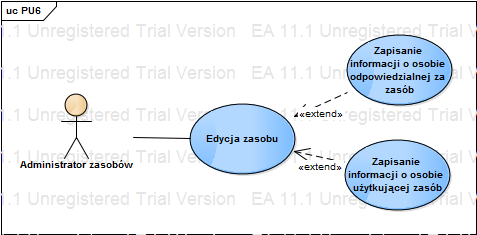
\includegraphics[scale=0.6]{img/diagrams/useCaseDiagrams/PU6.png}
	\caption{Diagram przypadków użycia PU6.1 i PU6.2 \label{fig:labelUCPU6}}
\end{figure}

\subsubsection{PU6.1 Zapisanie informacji o osobie odpowiedzialnej za zasób}
\myparagraph{Opis}
Przypadek zapisywania informacji o osobie, która odpowiada za zasób.

\myparagraph{Aktorzy}
Administrator zasobów.

\myparagraph{Warunki wstępne}
\begin{itemize}
\item Użytkownik jest zalogowany w systemie.
\item Osoba odpowiedzialna za zasób znajduje się w bazie pracowników.
\end{itemize}

\myparagraph{Warunki końcowe}
\begin{itemize}
\item Do systemu katalogowego została zapisana informacja o osobie odpowiedzialnej za zasób.
\end{itemize}

\myparagraph{Przebieg podstawowy}
\begin{enumerate}
	\item \label{pu6.1:1} Aktor wyszukuje zasób zgodnie z \ref{pu1}
	\item \label{pu6.1:2} Aktor wybiera sprzęt oraz wciska przycisk ,,Edytuj''.
	\item System prezentuje okno edycji zasobu.
	\item Aktor wybiera pracownika odpowiedzialnego za zasób ze zbioru wszystkich pracowników, mających uprawnienia do bycia odpowiedzialnym nad typem edytowanego zasobu.
	\item Aktor wciska przycisk „Zapisz”.
	\item System wyświetla potwierdzenie zmiany danych zasobu.
\end{enumerate}

\myparagraph{Alternatywne przebiegi zdarzeń}
\begin{enumerate}
	\item Aktor nie posiada uprawnień do edycji zasobu.
	\begin{enumerate}[label*=\arabic*.]
		\item Kroki \ref{pu6.1:1} - \ref{pu6.1:2} jak w przebiegu podstawowym.
		\item System wyświetla informację o braku uprawnień do edycji.
	\end{enumerate}
\end{enumerate}
\myparagraph{Sytuacje wyjątkowe}
Brak połączenia z siecią.

\begin{figure}[h!]
	\centering
	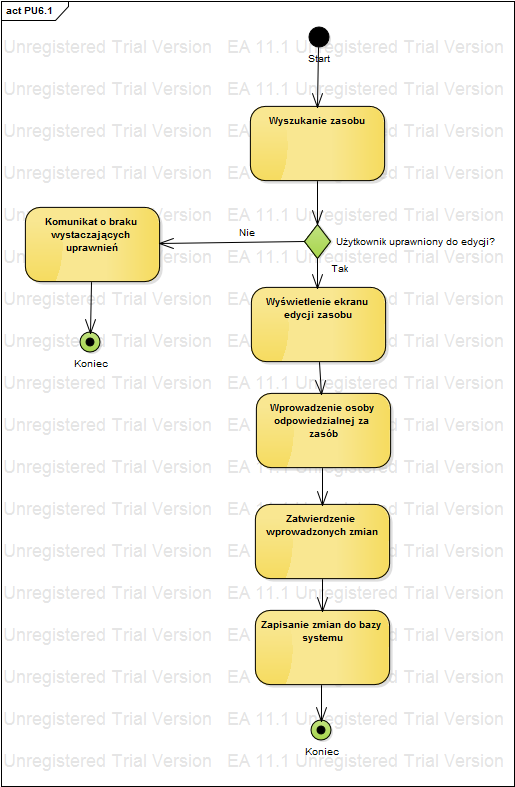
\includegraphics[scale=0.6]{img/diagrams/activityDiagrams/PU61}
	\caption{Diagram aktywności przypadku użycia PU6.1 \label{fig:labelADPU6.1}}
\end{figure}

\subsubsection{PU6.2 Zapisanie informacji o użytkowniku konkretnego zasobu}
\myparagraph{Opis}
Przypadek zapisywania informacji o użytkownikach zasobu.

\myparagraph{Aktorzy}
Administrator zasobów.

\myparagraph{Warunki wstępne}
\begin{itemize}
\item Użytkownik jest zalogowany w systemie.
\item Osoba odpowiedzialna za zasób znajduje się w bazie pracowników.
\end{itemize}

\myparagraph{Warunki końcowe}
\begin{itemize}
\item Do systemu katalogowego została zapisana informacja o osobie użytkującej zasób.
\end{itemize}

\myparagraph{Przebieg podstawowy}
\begin{enumerate}
	\item \label{pu6.2:1} Aktor wyszukuje sprzęt zgodnie z \ref{pu1}
	\item \label{pu6.2:2} Aktor wybiera sprzęt oraz wciska przycisk ,,Edytuj''.
	\item System prezentuje okno edycji zasobu.
	\item Aktor modyfikuje listę użytkowników użytkujących dany zasób.
	\item Aktor wciska przycisk „Zapisz”.
	\item System wyświetla potwierdzenie zmiany danych zasobu.
\end{enumerate}

\myparagraph{Alternatywne przebiegi zdarzeń}
\begin{enumerate}
	\item Aktor nie posiada uprawnień do edycji zasobu.
	\begin{enumerate}[label*=\arabic*.]
		\item Kroki \ref{pu6.2:1} - \ref{pu6.2:2} jak w przebiegu podstawowym.
		\item System wyświetla informację o braku uprawnień do edycji.
	\end{enumerate}
\end{enumerate}

\myparagraph{Sytuacje wyjątkowe}
Brak połączenia z siecią.

\begin{figure}[h!]
	\centering
	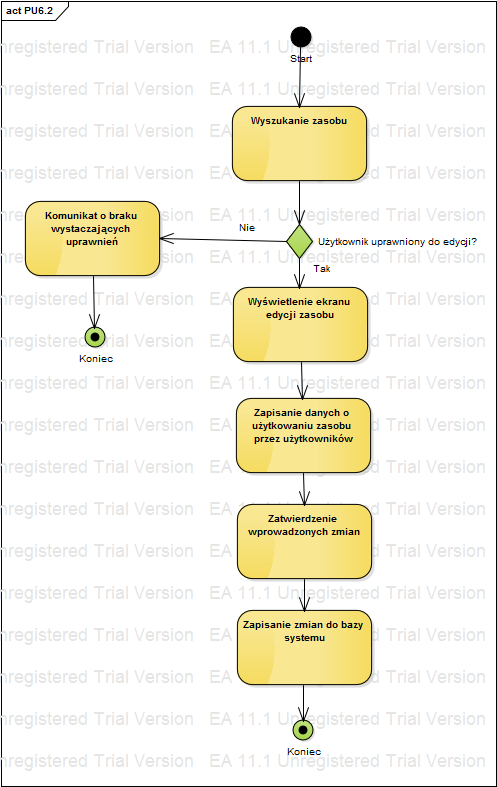
\includegraphics[scale=0.6]{img/diagrams/activityDiagrams/PU62}
	\caption{Diagram aktywności przypadku użycia PU6.2 \label{fig:labelADPU6.2}}
\end{figure}

\subsection{PU7 Obliczanie statystyk} \label{pu7}
\begin{figure}[h!]
	\centering
	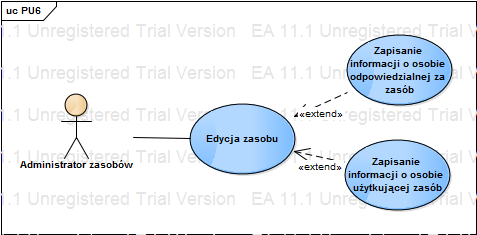
\includegraphics[scale=0.6]{img/diagrams/useCaseDiagrams/PU6.png}
	\caption{Diagram przypadków użycia PU6.1 i PU6.2 \label{fig:labelUCPU6}}
\end{figure}

\subsubsection{PU7.1 Prezentacja zakupów konkretnych zasobów w poszczególnych latach}
\myparagraph{Opis}
Przypadek prezentowania statystyk dotyczących ilości zakupów zasobów wybranych przez użytkownika w latach wybranych przez użytkownika.

\myparagraph{Aktorzy}
Menadżer.

\myparagraph{Warunki wstępne}
\begin{itemize}
\item Użytkownik jest zalogowany w systemie.
\end{itemize}

\myparagraph{Warunki końcowe}
\begin{itemize}
\item Użytkownik otrzymuje prezentacje statystyk dotyczących zakupów zasobów w latach.
\end{itemize}

\myparagraph{Przebieg podstawowy}
\begin{enumerate}
	\item \label{pu7.1:1} Aktor wybiera ikone generowania statystyk.
	\item System prezentuje dostępne typy raportów.
	\item \label{pu7.2:2} Aktor wybiera prezentacje statystyk dotyczących zakupów zasobów w latach.
	\item System prezentuje okno parametrów raportu.
	\item Aktor wybiera zasoby dla których mają być obliczane statystyki oraz wybiera lata dla których mają być wygenerowany raport.
	\item Aktor wciska przycisk „Generuj”.
	\item System wyświetla prezentacje statystyk.
\end{enumerate}

\myparagraph{Alternatywne przebiegi zdarzeń}
\begin{enumerate}
	\item Aktor nie posiada uprawnień generowania raportów.
	\begin{enumerate}[label*=\arabic*.]
		\item Krok \ref{pu6.1:1} jak w przebiegu podstawowym.
		\item System wyświetla informację o braku uprawnień do generowania raportów.
	\end{enumerate}
\end{enumerate}

\myparagraph{Sytuacje wyjątkowe}
Brak połączenia z siecią.

\begin{figure}[h!]
	\centering
	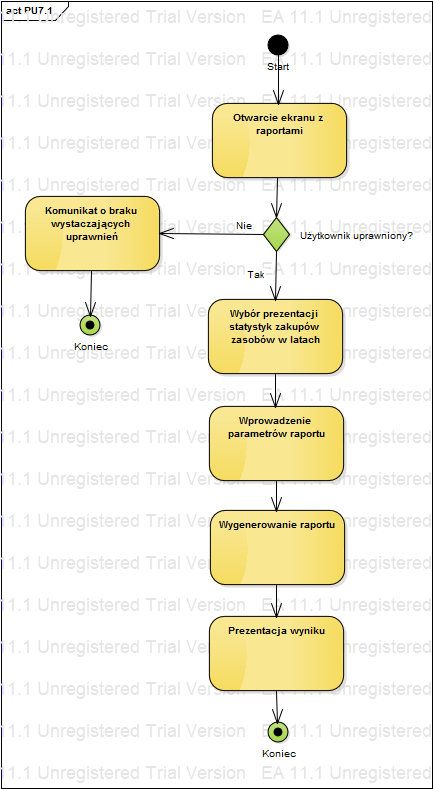
\includegraphics[scale=0.6]{img/diagrams/activityDiagrams/PU71.png}
	\caption{Diagram aktywności przypadku użycia PU7.1 \label{fig:labelADPU7.1}}
\end{figure}

\subsubsection{PU7.2.1 Prezentacja ilości zakupionych zasobów w poszczególnych działach}
\myparagraph{Opis}
Przypadek prezentowania statystyk dotyczących ilości zakupów zasobów wybranych przez użytkownika w działach wybranych przez użytkownika.

\myparagraph{Aktorzy}
Menadżer.

\myparagraph{Warunki wstępne}
\begin{itemize}
\item Użytkownik jest zalogowany w systemie.
\end{itemize}

\myparagraph{Warunki końcowe}
\begin{itemize}
\item Użytkownik otrzymuje prezentacje statystyk dotyczących zakupów zasobów w działach.
\end{itemize}

\myparagraph{Przebieg podstawowy}
\begin{enumerate}
	\item \label{pu7.2.1:1} Aktor wybiera ikone generowania statystyk.
	\item System prezentuje dostępne typy raportów.
	\item \label{pu7.2.1:2} Aktor wybiera prezentacje statystyk dotyczących zakupów zasobów w działach.
	\item System prezentuje okno parametrów raportu.
	\item Aktor wybiera zasoby dla których mają być obliczane statystyki oraz wybiera działy dla których mają być wygenerowany raport.
	\item Aktor wciska przycisk „Generuj”.
	\item System wyświetla prezentacje statystyk.
\end{enumerate}

\myparagraph{Alternatywne przebiegi zdarzeń}
\begin{enumerate}
	\item Aktor nie posiada uprawnień generowania raportów.
	\begin{enumerate}[label*=\arabic*.]
		\item Krok \ref{pu6.1:1} jak w przebiegu podstawowym.
		\item System wyświetla informację o braku uprawnień do generowania raportów.
	\end{enumerate}
\end{enumerate}

\myparagraph{Sytuacje wyjątkowe}
Brak połączenia z siecią.

\begin{figure}[h!]
	\centering
	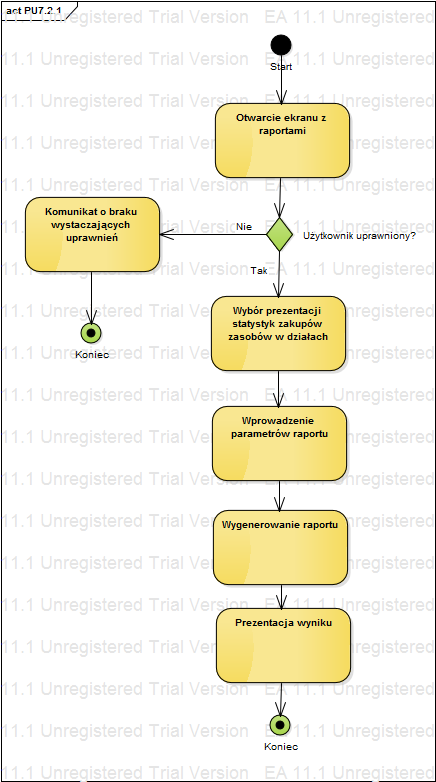
\includegraphics[scale=0.6]{img/diagrams/activityDiagrams/PU721}
	\caption{Diagram aktywności przypadku użycia PU7.2.1 \label{fig:labelADPU7.2.1}}
\end{figure}

\subsubsection{PU7.2.2 Prezentacja ilości używanych zasobów w poszczególnych działach}
\myparagraph{Opis}
Przypadek prezentowania statystyk dotyczących ilości używanych zasobów wybranych przez użytkownika w działach wybranych przez użytkownika.

\myparagraph{Aktorzy}
Menadżer.

\myparagraph{Warunki wstępne}
\begin{itemize}
\item Użytkownik jest zalogowany w systemie.
\end{itemize}

\myparagraph{Warunki końcowe}
\begin{itemize}
\item Użytkownik otrzymuje prezentacje statystyk dotyczących użycia zasobów w działach.
\end{itemize}

\myparagraph{Przebieg podstawowy}
\begin{enumerate}
	\item \label{pu7.2.2:1} Aktor wybiera ikone generowania statystyk.
	\item System prezentuje dostępne typy raportów.
	\item \label{pu7.2.2:2} Aktor wybiera prezentacje statystyk dotyczących użycia zasobów w działach.
	\item System prezentuje okno parametrów raportu.
	\item Aktor wybiera zasoby dla których mają być obliczane statystyki oraz wybiera działy dla których mają być wygenerowany raport.
	\item Aktor wciska przycisk „Generuj”.
	\item System wyświetla prezentacje statystyk.
\end{enumerate}

\myparagraph{Alternatywne przebiegi zdarzeń}
\begin{enumerate}
	\item Aktor nie posiada uprawnień generowania raportów.
	\begin{enumerate}[label*=\arabic*.]
		\item Krok \ref{pu6.1:1} jak w przebiegu podstawowym.
		\item System wyświetla informację o braku uprawnień do generowania raportów.
	\end{enumerate}
\end{enumerate}

\myparagraph{Sytuacje wyjątkowe}
Brak połączenia z siecią.

\begin{figure}[h!]
	\centering
	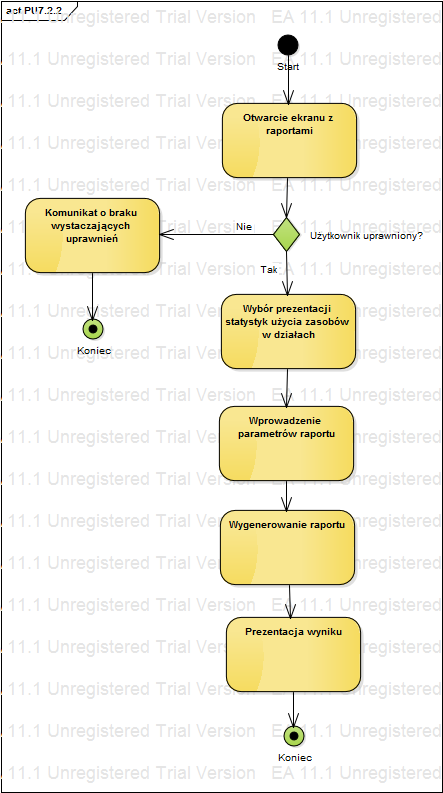
\includegraphics[scale=0.6]{img/diagrams/activityDiagrams/PU722}
	\caption{Diagram aktywności przypadku użycia PU7.2.2 \label{fig:labelADPU7.2.2}}
\end{figure}

\subsubsection{PU7.2.3 Prezentacja ilości napraw zasobów w poszczególnych działach}
\myparagraph{Opis}
Przypadek prezentowania statystyk dotyczących ilości napraw zasobów wybranych przez użytkownika w działach wybranych przez użytkownika.

\myparagraph{Aktorzy}
Menadżer.

\myparagraph{Warunki wstępne}
\begin{itemize}
\item Użytkownik jest zalogowany w systemie.
\end{itemize}

\myparagraph{Warunki końcowe}
\begin{itemize}
\item Użytkownik otrzymuje prezentacje statystyk dotyczących napraw zasobów w działach.
\end{itemize}

\myparagraph{Przebieg podstawowy}
\begin{enumerate}
	\item \label{pu7.2.3:1} Aktor wybiera ikone generowania statystyk.
	\item System prezentuje dostępne typy raportów.
	\item \label{pu7.2.3:2} Aktor wybiera prezentacje statystyk dotyczących napraw zasobów w działach.
	\item System prezentuje okno parametrów raportu.
	\item Aktor wybiera zasoby dla których mają być obliczane statystyki oraz wybiera działy dla których mają być wygenerowany raport.
	\item Aktor wciska przycisk „Generuj”.
	\item System wyświetla prezentacje statystyk.
\end{enumerate}

\myparagraph{Alternatywne przebiegi zdarzeń}
\begin{enumerate}
	\item Aktor nie posiada uprawnień generowania raportów.
	\begin{enumerate}[label*=\arabic*.]
		\item Krok \ref{pu6.1:1} jak w przebiegu podstawowym.
		\item System wyświetla informację o braku uprawnień do generowania raportów.
	\end{enumerate}
\end{enumerate}

\myparagraph{Sytuacje wyjątkowe}
Brak połączenia z siecią.

\begin{figure}[h!]
	\centering
	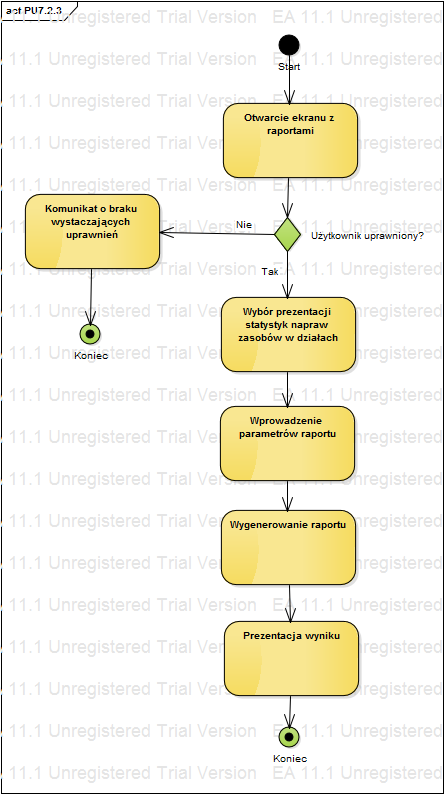
\includegraphics[scale=0.6]{img/diagrams/activityDiagrams/PU723}
	\caption{Diagram aktywności przypadku użycia PU7.2.3 \label{fig:labelADPU7.2.3}}
\end{figure}

\subsubsection{PU7.3.1 Prezentacja ilości zakupionych zasobów w poszczególnych placówkach}
\myparagraph{Opis}
Przypadek prezentowania statystyk dotyczących ilości zakupów zasobów wybranych przez użytkownika w placówkach wybranych przez użytkownika.

\myparagraph{Aktorzy}
Menadżer.

\myparagraph{Warunki wstępne}
\begin{itemize}
\item Użytkownik jest zalogowany w systemie.
\end{itemize}

\myparagraph{Warunki końcowe}
\begin{itemize}
\item Użytkownik otrzymuje prezentacje statystyk dotyczących zakupu zasobów w placówkach.
\end{itemize}

\myparagraph{Przebieg podstawowy}
\begin{enumerate}
	\item \label{pu7.3.1:1} Aktor wybiera ikone generowania statystyk.
	\item System prezentuje dostępne typy raportów.
	\item \label{pu7.3.1:2} Aktor wybiera prezentacje statystyk dotyczących zakupów zasobów w placówkach.
	\item System prezentuje okno parametrów raportu.
	\item Aktor wybiera zasoby dla których mają być obliczane statystyki oraz wybiera placówki dla których mają być wygenerowany raport.
	\item Aktor wciska przycisk „Generuj”.
	\item System wyświetla prezentacje statystyk.
\end{enumerate}

\myparagraph{Alternatywne przebiegi zdarzeń}
\begin{enumerate}
	\item Aktor nie posiada uprawnień generowania raportów.
	\begin{enumerate}[label*=\arabic*.]
		\item Krok \ref{pu6.1:1} jak w przebiegu podstawowym.
		\item System wyświetla informację o braku uprawnień do generowania raportów.
	\end{enumerate}
\end{enumerate}

\myparagraph{Sytuacje wyjątkowe}
Brak połączenia z siecią.

\begin{figure}[h!]
	\centering
	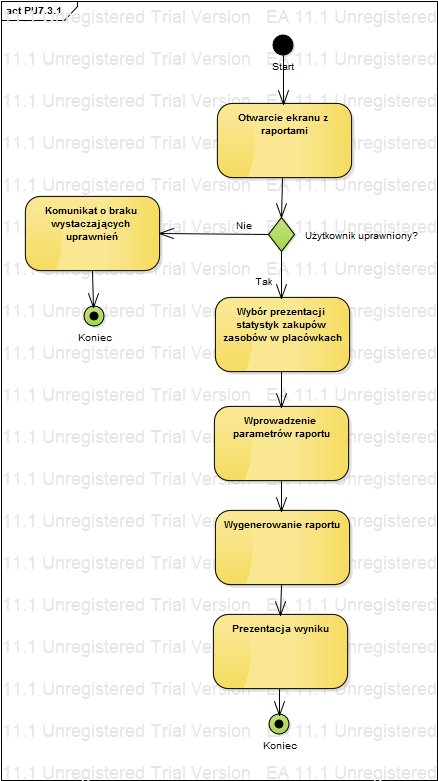
\includegraphics[scale=0.6]{img/diagrams/activityDiagrams/PU731}
	\caption{Diagram aktywności przypadku użycia PU7.3.1 \label{fig:labelADPU7.3.1}}
\end{figure}

\subsubsection{PU7.3.2 Prezentacja ilości używanych zasobów w poszczególnych placówkach}
\myparagraph{Opis}
Przypadek prezentowania statystyk dotyczących ilości używanych zasobów wybranych przez użytkownika w placówkach wybranych przez użytkownika.

\myparagraph{Aktorzy}
Menadżer.

\myparagraph{Warunki wstępne}
\begin{itemize}
\item Użytkownik jest zalogowany w systemie.
\end{itemize}

\myparagraph{Warunki końcowe}
\begin{itemize}
\item Użytkownik otrzymuje prezentacje statystyk dotyczących użycia zasobów w placówkach.
\end{itemize}

\myparagraph{Przebieg podstawowy}
\begin{enumerate}
	\item \label{pu7.3.2:1} Aktor wybiera ikone generowania statystyk.
	\item System prezentuje dostępne typy raportów.
	\item \label{pu7.3.2:2} Aktor wybiera prezentacje statystyk dotyczących użycia zasobów w placówkach.
	\item System prezentuje okno parametrów raportu.
	\item Aktor wybiera zasoby dla których mają być obliczane statystyki oraz wybiera placówki dla których mają być wygenerowany raport.
	\item Aktor wciska przycisk „Generuj”.
	\item System wyświetla prezentacje statystyk.
\end{enumerate}

\myparagraph{Alternatywne przebiegi zdarzeń}
\begin{enumerate}
	\item Aktor nie posiada uprawnień generowania raportów.
	\begin{enumerate}[label*=\arabic*.]
		\item Krok \ref{pu6.1:1} jak w przebiegu podstawowym.
		\item System wyświetla informację o braku uprawnień do generowania raportów.
	\end{enumerate}
\end{enumerate}

\myparagraph{Sytuacje wyjątkowe}
Brak połączenia z siecią.

\begin{figure}[h!]
	\centering
	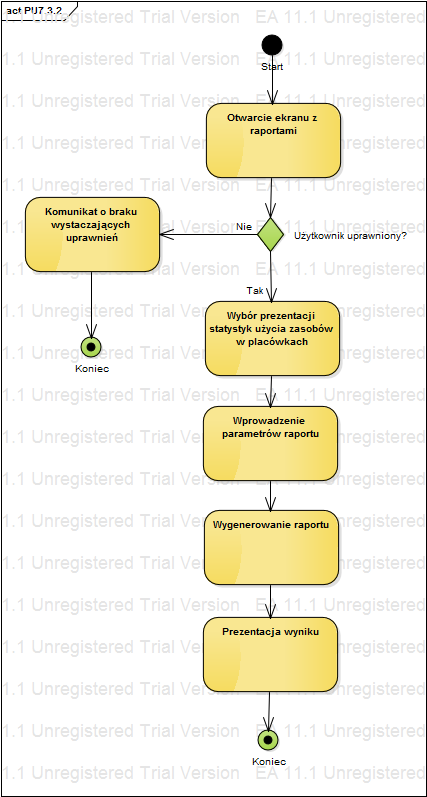
\includegraphics[scale=0.6]{img/diagrams/activityDiagrams/PU732}
	\caption{Diagram aktywności przypadku użycia PU7.3.2 \label{fig:labelADPU7.3.2}}
\end{figure}

\subsubsection{PU7.3.3 Prezentacja ilości napraw zasobów w poszczególnych placówkach}
\myparagraph{Opis}
Przypadek prezentowania statystyk dotyczących ilości napraw zasobów wybranych przez użytkownika w placówkach wybranych przez użytkownika.

\myparagraph{Aktorzy}
Menadżer.

\myparagraph{Warunki wstępne}
\begin{itemize}
\item Użytkownik jest zalogowany w systemie.
\end{itemize}

\myparagraph{Warunki końcowe}
\begin{itemize}
\item Użytkownik otrzymuje prezentacje statystyk dotyczących napraw zasobów w placówkach.
\end{itemize}

\myparagraph{Przebieg podstawowy}
\begin{enumerate}
	\item \label{pu7.3.3:1} Aktor wybiera ikone generowania statystyk.
	\item System prezentuje dostępne typy raportów.
	\item \label{pu7.3.3:2} Aktor wybiera prezentacje statystyk dotyczących napraw zasobów w placówkach.
	\item System prezentuje okno parametrów raportu.
	\item Aktor wybiera zasoby dla których mają być obliczane statystyki oraz wybiera działy dla których mają być wygenerowany raport.
	\item Aktor wciska przycisk „Generuj”.
	\item System wyświetla prezentacje statystyk.
\end{enumerate}

\myparagraph{Alternatywne przebiegi zdarzeń}
\begin{enumerate}
	\item Aktor nie posiada uprawnień generowania raportów.
	\begin{enumerate}[label*=\arabic*.]
		\item Krok \ref{pu6.1:1} jak w przebiegu podstawowym.
		\item System wyświetla informację o braku uprawnień do generowania raportów.
	\end{enumerate}
\end{enumerate}

\myparagraph{Sytuacje wyjątkowe}
Brak połączenia z siecią.

\begin{figure}[h!]
	\centering
	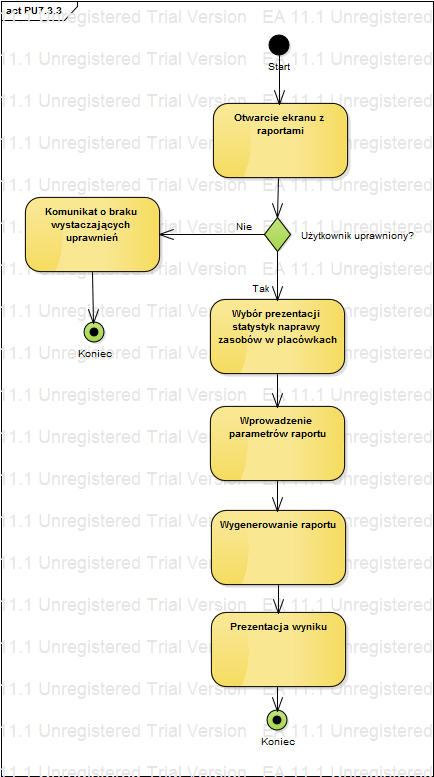
\includegraphics[scale=0.6]{img/diagrams/activityDiagrams/PU733}
	\caption{Diagram aktywności przypadku użycia PU7.3.3 \label{fig:labelADPU7.3.3}}
\end{figure}

\subsection{PU8 Rejestracja informacji dotyczącej miejsca zakupu} \label{pu8}
\begin{figure}[h!]
	\centering
	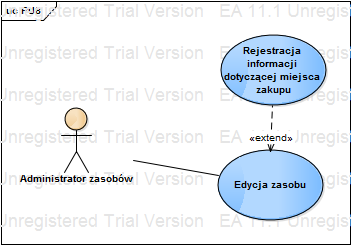
\includegraphics[scale=0.6]{img/diagrams/useCaseDiagrams/PU8}
	\caption{Diagram przypadków użycia PU8 \label{fig:labelUCPU8}}
\end{figure}

\myparagraph{Opis}
Przypadek rejestracji miejsca zakupu zasobu.

\myparagraph{Aktorzy}
Administrator zasobów.

\myparagraph{Warunki wstępne}
\begin{itemize}
\item Użytkownik jest zalogowany w systemie.
\item Zasób jest już wprowadzony do bazy systemu.
\end{itemize}

\myparagraph{Warunki końcowe}
\begin{itemize}
\item Do systemu katalogowego została zapisana informacja dotycząca miejsca zakupu zasobu.
\end{itemize}

\myparagraph{Przebieg podstawowy}
\begin{enumerate}
	\item \label{pu8:1} Aktor wyszukuje zasób zgodnie z \ref{pu1}
	\item \label{pu8:2} Aktor wybiera zasób oraz wciska przycisk ,,Edytuj''.
	\item System prezentuje okno edycji zasobu.
	\item Aktor wprowadza informacje dotyczącą miejsca zakupu zasobu.
	\item Aktor wciska przycisk „Zapisz”.
	\item System wyświetla potwierdzenie zmiany danych zasobu.
\end{enumerate}

\myparagraph{Alternatywne przebiegi zdarzeń}
\begin{enumerate}
	\item Aktor nie posiada uprawnień do edycji zasobu.
	\begin{enumerate}[label*=\arabic*.]
		\item Kroki \ref{pu8:1} - \ref{pu8:2} jak w przebiegu podstawowym.
		\item System wyświetla informację o braku uprawnień do edycji.
	\end{enumerate}
\end{enumerate}

\myparagraph{Sytuacje wyjątkowe}
Brak połączenia z siecią.

\begin{figure}[h!]
	\centering
	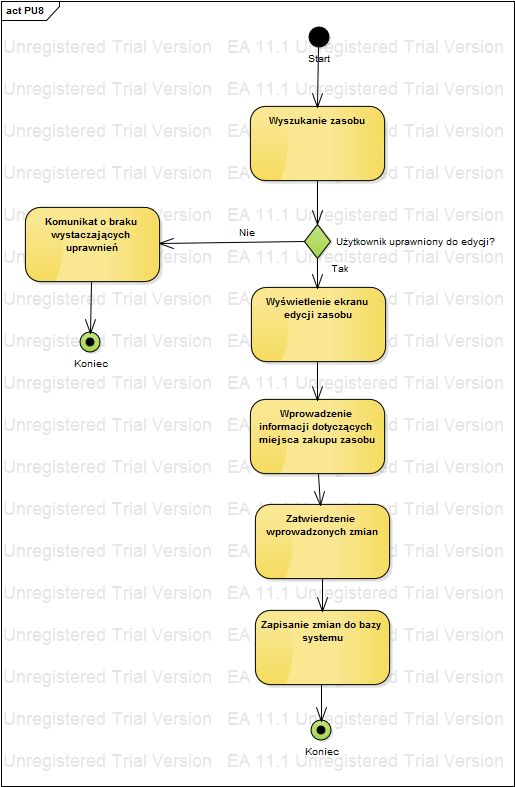
\includegraphics[scale=0.6]{img/diagrams/activityDiagrams/PU8.png}
	\caption{Diagram aktywności przypadku użycia PU8 \label{fig:labelADPU8}}
\end{figure}

\subsection{PU9 Historia napraw sprzętu} \label{pu9}
\begin{figure}[h!]
	\centering
	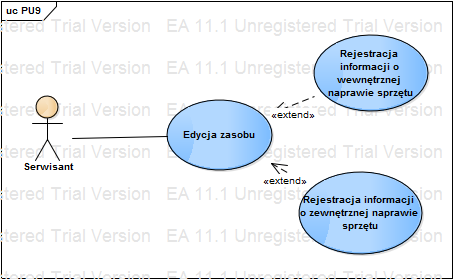
\includegraphics[scale=0.6]{img/diagrams/useCaseDiagrams/PU9.png}
	\caption{Diagram przypadków użycia PU9.1 i PU9.2 \label{fig:labelUCPU9}}
\end{figure}

\subsubsection{PU9.1 Rejestracja informacji o wewnętrznej naprawie sprzętu}
\myparagraph{Opis}
Przypadek rejestracji informacji naprawie sprzętu dokonanej wewnątrz firmy.

\myparagraph{Aktorzy}
Serwisant.

\myparagraph{Warunki wstępne}
\begin{itemize}
\item Użytkownik jest zalogowany w systemie.
\item Sprzęt jest już wprowadzony do bazy systemu.
\end{itemize}

\myparagraph{Warunki końcowe}
\begin{itemize}
\item Do systemu katalogowego została zapisana informacja dotycząca wewnętrznej naprawy sprzętu.
\end{itemize}

\myparagraph{Przebieg podstawowy}
\begin{enumerate}
	\item \label{pu9.1:1} Aktor wyszukuje sprzęt zgodnie z \ref{pu1}
	\item \label{pu9.1:2} Aktor wybiera sprzęt oraz wciska przycisk ,,Edytuj''.
	\item System prezentuje okno edycji sprzętu.
	\item \label{pu9.1:4} Aktor wprowadza informacje o przeprowadzonej wewnętrznej naprawie sprzętu.
	\item Aktor wciska przycisk „Zapisz”.
	\item System wyświetla potwierdzenie zmiany danych sprzętu.
\end{enumerate}

\myparagraph{Alternatywne przebiegi zdarzeń}
\begin{enumerate}
	\item Aktor nie posiada uprawnień do edycji sprzętu.
	\begin{enumerate}[label*=\arabic*.]
		\item Kroki \ref{pu9.1:1} - \ref{pu9.1:2} jak w przebiegu podstawowym.
		\item System wyświetla informację o braku uprawnień do edycji.
	\end{enumerate}
	\item Niepoprawny okres przebywania w naprawie.
	\begin{enumerate}[label*=\arabic*.]
		\item Kroki \ref{pu9.1:1} - \ref{pu9.1:4} jak w przebiegu podstawowym.
		\item System wyświetla informację o nakładaniu się okresów naprawy z innym wpisem o naprawie.
	\end{enumerate}
\end{enumerate}

\myparagraph{Sytuacje wyjątkowe}
Brak połączenia z siecią.

\begin{figure}[h!]
	\centering
	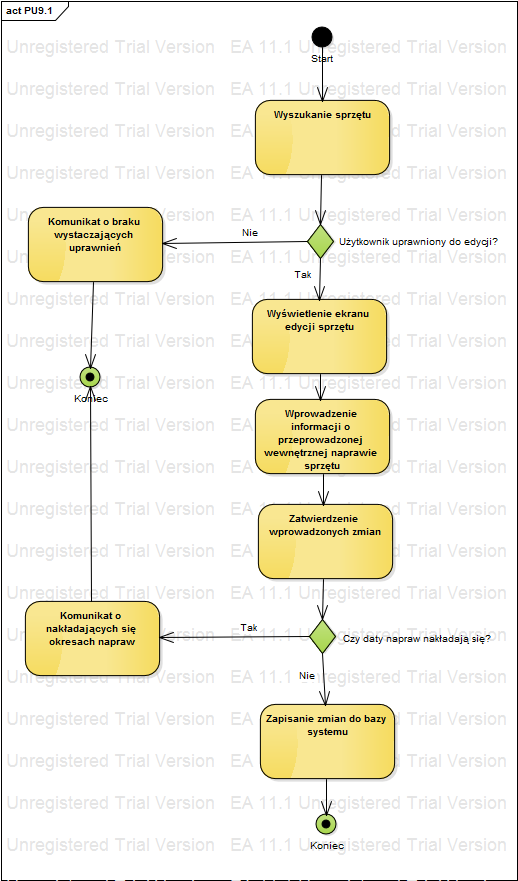
\includegraphics[scale=0.6]{img/diagrams/activityDiagrams/PU91}
	\caption{Diagram aktywności przypadku użycia PU9.1 \label{fig:labelADPU9.1}}
\end{figure}

\subsubsection{PU9.2 Rejestracja informacji o zewnętrznej naprawie sprzętu}
\myparagraph{Opis}
Przypadek rejestracji informacji naprawie sprzętu dokonanej w firmie zewnętrznej.

\myparagraph{Aktorzy}
Serwisant.

\myparagraph{Warunki wstępne}
\begin{itemize}
\item Użytkownik jest zalogowany w systemie.
\item Sprzęt jest już wprowadzony do bazy systemu.
\end{itemize}

\myparagraph{Warunki końcowe}
\begin{itemize}
\item Do systemu katalogowego została zapisana informacja dotycząca zewnętrznej naprawy sprzętu.
\end{itemize}

\myparagraph{Przebieg podstawowy}
\begin{enumerate}
	\item \label{pu9.2:1} Aktor wyszukuje sprzęt zgodnie z \ref{pu1}
	\item \label{pu9.2:2} Aktor wybiera sprzęt oraz wciska przycisk ,,Edytuj''.
	\item System prezentuje okno edycji sprzętu.
	\item \label{pu9.2:4} Aktor wprowadza informacje o przeprowadzonej zewnętrznej naprawie sprzętu.
	\item Aktor wciska przycisk „Zapisz”.
	\item System wyświetla potwierdzenie zmiany danych sprzętu.
\end{enumerate}

\myparagraph{Alternatywne przebiegi zdarzeń}
\begin{enumerate}
	\item Aktor nie posiada uprawnień do edycji sprzętu.
	\begin{enumerate}[label*=\arabic*.]
		\item Kroki \ref{pu9.2:1} - \ref{pu9.2:2} jak w przebiegu podstawowym.
		\item System wyświetla informację o braku uprawnień do edycji.
	\end{enumerate}
	\item Niepoprawny okres przebywania w naprawie.
	\begin{enumerate}[label*=\arabic*.]
		\item Kroki \ref{pu9.2:1} - \ref{pu9.2:4} jak w przebiegu podstawowym.
		\item System wyświetla informację o nakładaniu się okresów naprawy z innym wpisem o naprawie.
	\end{enumerate}
\end{enumerate}

\myparagraph{Sytuacje wyjątkowe}
Brak połączenia z siecią.

\begin{figure}[h!]
	\centering
	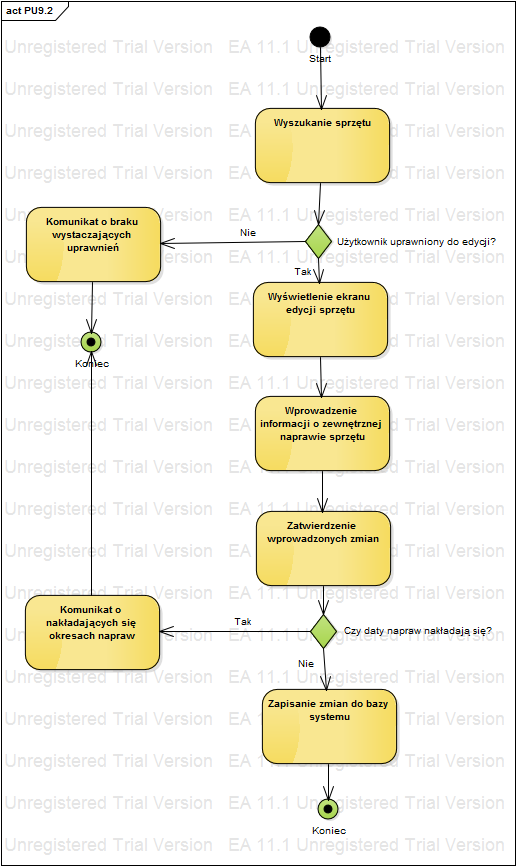
\includegraphics[scale=0.6]{img/diagrams/activityDiagrams/PU92}
	\caption{Diagram aktywności przypadku użycia PU9.2 \label{fig:labelADPU9.2}}
\end{figure}

\subsection{PU10 Rejestracja aktualizacji oprogramowania} \label{pu10}
\begin{figure}[h!]
	\centering
	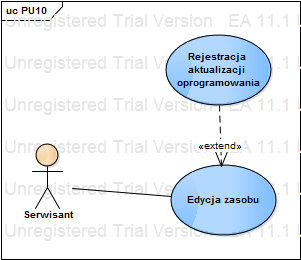
\includegraphics[scale=0.6]{img/diagrams/useCaseDiagrams/PU10}
	\caption{Diagram przypadków użycia PU10 \label{fig:labelUCPU10}}
\end{figure}

\myparagraph{Opis}
Przypadek rejestracji instalacji aktualizacji oprogramowania.

\myparagraph{Aktorzy}
Serwisant.

\myparagraph{Warunki wstępne}
\begin{itemize}
\item Użytkownik jest zalogowany w systemie.
\item Oprogramowanie jest już wprowadzone do bazy systemu.
\end{itemize}

\myparagraph{Warunki końcowe}
\begin{itemize}
\item Do systemu katalogowego została zapisana informacja dotycząca instalacji aktualizacji oprogramowania.
\end{itemize}

\myparagraph{Przebieg podstawowy}
\begin{enumerate}
	\item \label{pu10:1} Aktor wyszukuje oprogramowanie zgodnie z \ref{pu1}
	\item \label{pu10:2} Aktor wybiera oprogramowanie oraz wciska przycisk ,,Edytuj''.
	\item System prezentuje okno edycji oprogramowania.
	\item \label{pu10:4} Aktor wprowadza informacje o przeprowadzonej instalacji aktualizacji oprogramowania.
	\item Aktor wciska przycisk „Zapisz”.
	\item System wyświetla potwierdzenie zmiany danych oprogramowania.
\end{enumerate}

\myparagraph{Alternatywne przebiegi zdarzeń}
\begin{enumerate}
	\item Aktor nie posiada uprawnień do edycji oprogramowania.
	\begin{enumerate}[label*=\arabic*.]
		\item Kroki \ref{pu10:1} - \ref{pu10:2} jak w przebiegu podstawowym.
		\item System wyświetla informację o braku uprawnień do edycji.
	\end{enumerate}
	\item Aktualizacja oprogramowania została już przeprowadzona.
	\begin{enumerate}[label*=\arabic*.]
		\item Kroki \ref{pu10:1} - \ref{pu10:4} jak w przebiegu podstawowym.
		\item System wyświetla informację o tym, że wprowadzana aktualizacja została już przeprowadzona.
	\end{enumerate}
\end{enumerate}

\myparagraph{Sytuacje wyjątkowe}
Brak połączenia z siecią.

\begin{figure}[h!]
	\centering
	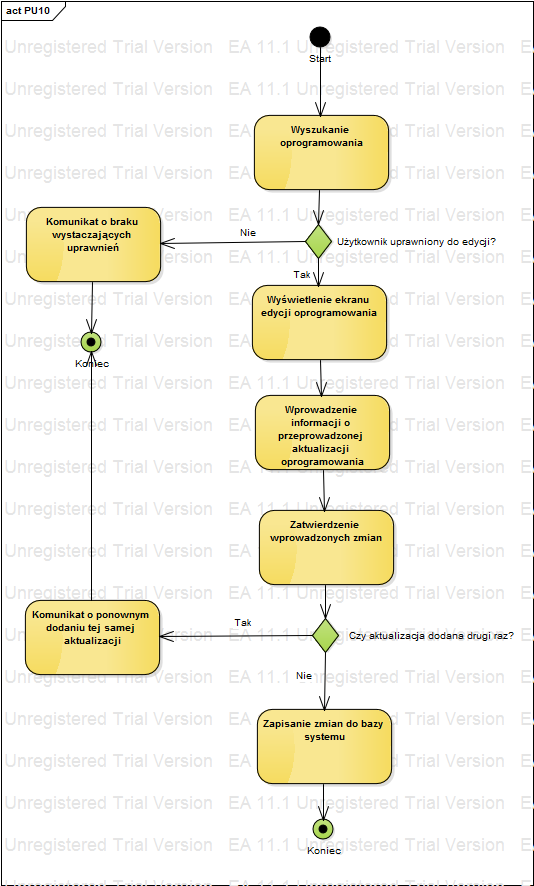
\includegraphics[scale=0.6]{img/diagrams/activityDiagrams/PU10.png}
	\caption{Diagram aktywności przypadku użycia PU10 \label{fig:labelADPU10}}
\end{figure}

\subsection{PU11 Rejestracja operacji serwisowej} \label{pu11}
\begin{figure}[h!]
	\centering
	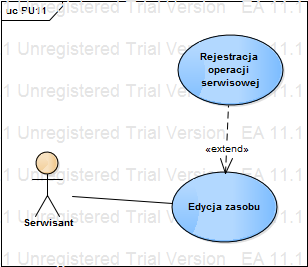
\includegraphics[scale=0.6]{img/diagrams/useCaseDiagrams/PU11.png}
	\caption{Diagram przypadków użycia PU11 \label{fig:labelUCPU11}}
\end{figure}

\myparagraph{Opis}
Przypadek rejestracji faktu serwisowania sprzętu.

\myparagraph{Aktorzy}
Serwisant.

\myparagraph{Warunki wstępne}
\begin{itemize}
\item Serwisant zalogowany w systemie.
\item Sprzęt jest już wprowadzony do bazy systemu.
\end{itemize}

\myparagraph{Warunki końcowe}
\begin{itemize}
\item Do systemu katalogowego została zapisana informacja dotycząca przeprowadzonej operacji serwisowej.
\end{itemize}

\myparagraph{Przebieg podstawowy}
\begin{enumerate}
	\item \label{pu11:1} Aktor wyszukuje sprzęt zgodnie z \ref{pu1}
	\item \label{pu11:2} Aktor wybiera sprzęt oraz wciska przycisk ,,Edytuj''.
	\item System prezentuje okno edycji sprzęt.
	\item Aktor wprowadza informacje o przeprowadzonej operacji serwisowej.
	\item Aktor wciska przycisk „Zapisz”.
	\item System wyświetla potwierdzenie zmiany danych sprzętu.
\end{enumerate}

\myparagraph{Alternatywne przebiegi zdarzeń}
\begin{enumerate}
	\item Aktor nie posiada uprawnień do edycji sprzętu.
	\begin{enumerate}[label*=\arabic*.]
		\item Kroki \ref{pu11:1} - \ref{pu11:2} jak w przebiegu podstawowym.
		\item System wyświetla informację o braku uprawnień do edycji.
	\end{enumerate}
\end{enumerate}


\myparagraph{Sytuacje wyjątkowe}
Brak połączenia z siecią.

\begin{figure}[h!]
	\centering
	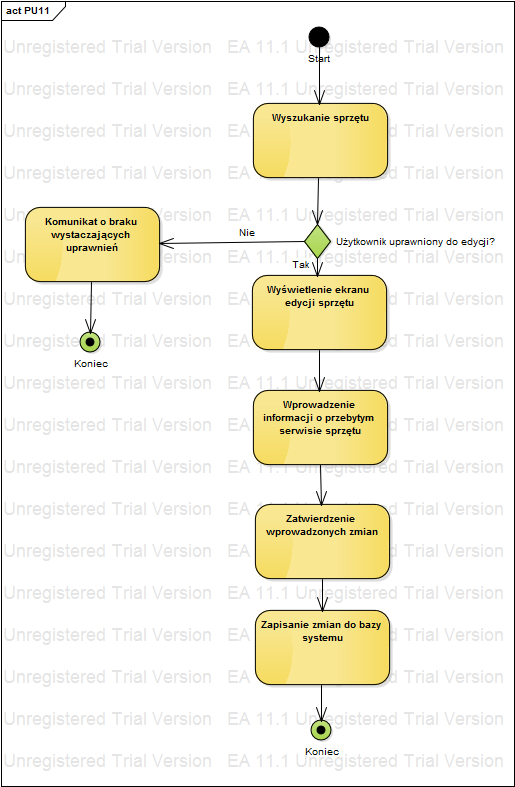
\includegraphics[scale=0.6]{img/diagrams/activityDiagrams/PU11.png}
	\caption{Diagram aktywności przypadku użycia PU11 \label{fig:labelADPU11}}
\end{figure}